\section{Uppgift 5}\label{sec:uppg05}

\subsection{Instruktioner}
\begin{Verbatim}[fontsize=small]
Skriv en klass Bilagare som representerar en bilägare. Klassen ska ha följande
tre instansvariabler:

namn (String), adress (String), bil (Personbil)

Instansvariablernas typer står inom parentes. I denna uppgift ska du även
använda dig av klassen Personbil som du skapade i uppgift 4. Efterson en
bilägare äger en bil så måste vi ha med instansvariabeln bil, som är en
referens till ett objekt av klassen Personbil.

I klassen Bilagare ska det finnas metoder för var och en av följande
operationer:

- returnera bilägarens namn
- returnera bilagarens adress
- bilägaren säljer sin bil (sätt instansvariabeln bil att ha värdet null)
- bilägaren köper ny bil (skicka som parameter med referensen till detta
  bil-objekt)
- skriv ut alla data om bilägarens bil, om han inte äger nån bil så ska
  valfritt meddelande (t.ex "Äger ingen bil för närvarande") istället
  skrivas ut. Metoden ska ha returtypen void.
- skriv ut bilägarens namn och adress.

Det ska naturligtvis finnas en konstruktor så att du kan initiera de tre
instansvariablerna.

Skriv ett testprogram som utför följande:

- Skapa två Personbils-objekt. Initiera objekten med valfria värden.
- Skapa ett Bilägare-objekt. Initiera objektet med valfria värden, ägarens
  bil måste dock vara någon av de två personbils-objekten.
- Skriv ut bilägarens namn och adress.
- Skriv ut data om bilägarens bil.
- Bilägaren säljer sin bil.
- Skriv ut data om bilägarens bil.
- Bilägaren köper en bil. Låt honom köpa någon av de två skapade
  personbils-objekten.
- Skriv ut data om bilägarens bil.
\end{Verbatim}


\subsection{Källkod}
\subsubsection{Lab3Uppg05.java}
\javacode{src/Lab3Uppg05/Lab3Uppg05.java}
\caption{Lab3Uppg05.java}
\label{src:uppg05}

\subsubsection{Bilagare.java}
\javacode{src/Lab3Uppg05/Bilagare.java}
\caption{Bilagare.java}
\label{src:bilagare}


\subsection{Skärmdump}
Se Figur~\ref{fig:uppg05-screenshot} för skärmdump på körning av koden i 
Sektion~\ref{src:uppg05}.

\begin{figure}[htbp]
    \centering
        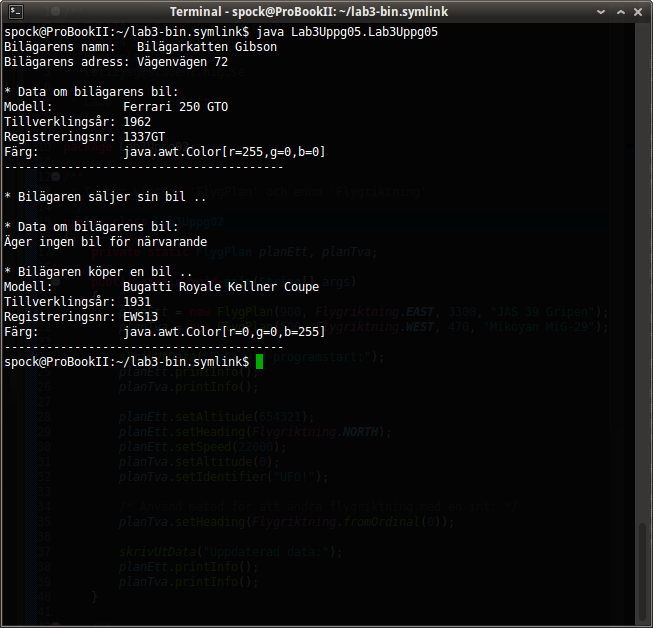
\includegraphics[width=\linewidth]{img/05.png}
    \caption{Körning av koden till Uppgift~\ref{sec:uppg05}}
    \label{fig:uppg05-screenshot}
\end{figure}

